
Given that the threshold of the detector is zero. Define a detector function $g$ such that
\begin{align}
g(Y) = 
\begin{cases}
+a & Y>0 \\
-a & Y<0
\end{cases}
\end{align}
It is given that $X \in \{ -a, a\}$ is a random variable.
\begin{align}
\therefore \Pr(X=a) = \Pr(X=-a) = \dfrac{1}{2}
\end{align}
Since the noise in the signal, $Z$ is chosen independently from a Gaussian distribution with mean $ \mu = \beta X$ and unit variance, it follows that
\begin{align}
F_Z(z) &= \int_{-\infty}^{z} \dfrac{1}{\sqrt{2\pi}} \exp \left( \dfrac{-(z - \beta X)^2}{2} \right) dz \\
&= \int_{-\infty}^{z - \beta X} \dfrac{1}{\sqrt{2\pi}} \exp \left( \dfrac{-z^2}{2} \right) dz \\
&= \int_{\beta X-z}^{\infty} \dfrac{1}{\sqrt{2\pi}} \exp \left( \dfrac{-z^2}{2} \right) dz \\
&= Q(\beta X - z) \label{eqn 2.0.7}
\end{align}
Also, it is easy to see that 
\begin{align}
Q(-v) = 1 - Q(v) \; \forall \; v \in \mathbb{R} \label{eqn 2.0.8}
\end{align}
The detector can record erroneous bits in the signal iff
\begin{align}
X>0 \; &, \; g(Y) = -a \; (\text{Call this BER}_{+a}) \text{ or}\\
X<0 \; &, \; g(Y) = a \; (\text{Call this BER}_{-a})
\end{align}
\begin{align}
\therefore \text{BER}_{+a} % &= \Pr(g(Y) = -a \;,\; X = a)\\
&= \Pr(g(Y) = -a \;|\; X = a) \Pr(X=a)\\
&= \Pr(Y < 0 \;|\; X = a) \Pr(X=a)\\
&= \dfrac{1}{2} \times \Pr(X+Z < 0 \;|\; X = a) \\
% &= \dfrac{1}{2} \times \Pr(a+Z < 0 \;|\; X = a) \\
% &= \dfrac{1}{2} \times \Pr(Z < -a \;|\; X = a) \\
&= \dfrac{1}{2} \times F_Z(-a)\\
&= \dfrac{1}{2} \times Q(\beta X + a) \; \text{ (From (\ref{eqn 2.0.7}))}\\
% &= \dfrac{1}{2} \times Q(a \beta + a)\\
&= \dfrac{1}{2} \times Q(a(1+\beta))
\end{align}
\begin{align}
\text{BER}_{-a} % &= \Pr(g(Y) = a \;,\; X = -a)\\
&= \Pr(g(Y) = a \;|\; X = -a) \Pr(X=-a)\\
&= \Pr(Y > 0 \;|\; X = -a) \Pr(X=-a)\\
&= \dfrac{1}{2} \times \Pr(X+Z > 0 \;|\; X = -a) \\
% &= \dfrac{1}{2} \times \Pr(Z-a > 0 \;|\; X = -a) \\
% &= \dfrac{1}{2} \times \Pr(Z > a \;|\; X = -a) \\
&= \dfrac{1}{2} \times \left( 1 - F_Z(a) \right) \\
&= \dfrac{1}{2} \times \left( 1 - Q(\beta X -a) \right) \; \text{ (From (\ref{eqn 2.0.7}))}\\
% &= \dfrac{1}{2} \times \left( 1 - Q(-a \beta -a) \right) \\
&= \dfrac{1}{2} \times Q(a(1+\beta)) \; \text{ (From (\ref{eqn 2.0.8}))}
\end{align}
\begin{align}
\therefore \text{BER} &= \text{BER}_{+a} + \text{BER}_{-a}\\
&= Q(a(1+\beta))
\end{align} 
\begin{figure}[!hbt]
    \centering
	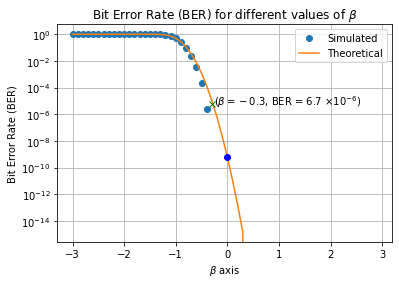
\includegraphics[width=\columnwidth]{solutions/ec/45/Figures/Figure_3.png}
    \caption{Theory vs Simulated plot of BER}
    \label{CDF_Y}
\end{figure}
When $\beta = 0$, it is given that 
\begin{align}
\text{BER} = Q(a) &= 10^{-8}
\end{align}
On computing, $Q(1) \approx 0.16$. Since $Q(a)<Q(1)$, it is easy to see that $a>1$ (as $Q(x)$ is a decreasing function)
\begin{align}
\therefore e^{-a^2 / 2} &= 10^{-8}\\
\Leftrightarrow a &\approx 6.069
\end{align}
When $\beta = -0.3$,
\begin{align}
\text{BER} = Q(a(1+\beta)) &= Q(6.069 \times (1-0.3))\\
&= Q(6.069 \times 0.7)\\
&= Q(4.249)\\
&\approx \exp (-\dfrac{4.249^2}{2})\\
&\approx 1.2 \times 10^{-4}
\end{align}
Therefore, when $\beta = -0.3$, BER is closest to $10^{-4}$ and option \ref{option C} is correct.

